% Options for packages loaded elsewhere
\PassOptionsToPackage{unicode}{hyperref}
\PassOptionsToPackage{hyphens}{url}
\documentclass[
]{article}
\usepackage{xcolor}
\usepackage[margin=1in]{geometry}
\usepackage{amsmath,amssymb}
\setcounter{secnumdepth}{5}
\usepackage{iftex}
\ifPDFTeX
  \usepackage[T1]{fontenc}
  \usepackage[utf8]{inputenc}
  \usepackage{textcomp} % provide euro and other symbols
\else % if luatex or xetex
  \usepackage{unicode-math} % this also loads fontspec
  \defaultfontfeatures{Scale=MatchLowercase}
  \defaultfontfeatures[\rmfamily]{Ligatures=TeX,Scale=1}
\fi
\usepackage{lmodern}
\ifPDFTeX\else
  % xetex/luatex font selection
\fi
% Use upquote if available, for straight quotes in verbatim environments
\IfFileExists{upquote.sty}{\usepackage{upquote}}{}
\IfFileExists{microtype.sty}{% use microtype if available
  \usepackage[]{microtype}
  \UseMicrotypeSet[protrusion]{basicmath} % disable protrusion for tt fonts
}{}
\makeatletter
\@ifundefined{KOMAClassName}{% if non-KOMA class
  \IfFileExists{parskip.sty}{%
    \usepackage{parskip}
  }{% else
    \setlength{\parindent}{0pt}
    \setlength{\parskip}{6pt plus 2pt minus 1pt}}
}{% if KOMA class
  \KOMAoptions{parskip=half}}
\makeatother
\usepackage{longtable,booktabs,array}
\usepackage{calc} % for calculating minipage widths
% Correct order of tables after \paragraph or \subparagraph
\usepackage{etoolbox}
\makeatletter
\patchcmd\longtable{\par}{\if@noskipsec\mbox{}\fi\par}{}{}
\makeatother
% Allow footnotes in longtable head/foot
\IfFileExists{footnotehyper.sty}{\usepackage{footnotehyper}}{\usepackage{footnote}}
\makesavenoteenv{longtable}
\usepackage{graphicx}
\makeatletter
\newsavebox\pandoc@box
\newcommand*\pandocbounded[1]{% scales image to fit in text height/width
  \sbox\pandoc@box{#1}%
  \Gscale@div\@tempa{\textheight}{\dimexpr\ht\pandoc@box+\dp\pandoc@box\relax}%
  \Gscale@div\@tempb{\linewidth}{\wd\pandoc@box}%
  \ifdim\@tempb\p@<\@tempa\p@\let\@tempa\@tempb\fi% select the smaller of both
  \ifdim\@tempa\p@<\p@\scalebox{\@tempa}{\usebox\pandoc@box}%
  \else\usebox{\pandoc@box}%
  \fi%
}
% Set default figure placement to htbp
\def\fps@figure{htbp}
\makeatother
\setlength{\emergencystretch}{3em} % prevent overfull lines
\providecommand{\tightlist}{%
  \setlength{\itemsep}{0pt}\setlength{\parskip}{0pt}}
\usepackage{bookmark}
\IfFileExists{xurl.sty}{\usepackage{xurl}}{} % add URL line breaks if available
\urlstyle{same}
\hypersetup{
  pdftitle={MCnebula2 workflow for LC-MS/MS dataset analysis},
  hidelinks,
  pdfcreator={LaTeX via pandoc}}

\title{MCnebula2 workflow for LC-MS/MS dataset analysis}
\author{}
\date{\vspace{-2.5em}}

\begin{document}
\maketitle

{
\setcounter{tocdepth}{3}
\tableofcontents
}
\section{data processing}\label{data-processing}

\section{Sample infomation and outlier detection}\label{sample-infomation-and-outlier-detection}

\begin{table}[!h]
\centering
\caption{\label{tab:unnamed-chunk-3}example}
\centering
\begin{tabular}[t]{ll}
\toprule
sample & group\\
\midrule
M1 & Model\\
M10 & Model\\
M11 & Model\\
M12 & Model\\
M13 & Model\\
\addlinespace
M2 & Model\\
M3 & Model\\
M4 & Model\\
M6 & Model\\
M7 & Model\\
\addlinespace
M8 & Model\\
Sham1 & Sham\\
Sham2 & Sham\\
Sham3 & Sham\\
Sham4 & Sham\\
\addlinespace
Sham5 & Sham\\
Sham6 & Sham\\
Sham7 & Sham\\
Sham8 & Sham\\
Sham9 & Sham\\
\bottomrule
\end{tabular}
\end{table}

\section{Missing value}\label{missing-value}

\begin{verbatim}
## Cluster size 3350 broken into 33 3317 
## Done cluster 33 
## Cluster size 3317 broken into 212 3105 
## Done cluster 212 
## Cluster size 3105 broken into 414 2691 
## Done cluster 414 
## Cluster size 2691 broken into 547 2144 
## Done cluster 547 
## Cluster size 2144 broken into 664 1480 
## Done cluster 664 
## Done cluster 1480 
## Done cluster 2144 
## Done cluster 2691 
## Done cluster 3105 
## Done cluster 3317
\end{verbatim}

\section{RSD}\label{rsd}

\pandocbounded{
\includegraphics[keepaspectratio]{QC_report_files/figure-latex/unnamed-chunk-5-1.pdf}} \pandocbounded{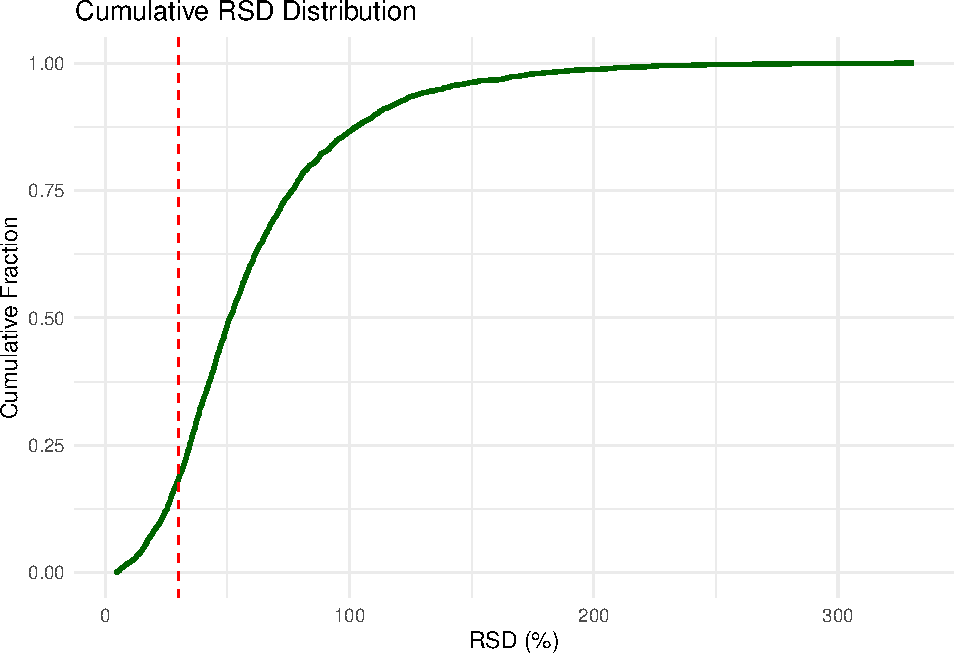
\includegraphics[keepaspectratio]{QC_report_files/figure-latex/unnamed-chunk-5-2.pdf}}

\section{intensity}\label{intensity}

\pandocbounded{
\includegraphics[keepaspectratio]{QC_report_files/figure-latex/unnamed-chunk-6-1.pdf}}

\section{correlation}\label{correlation}

\pandocbounded{
\includegraphics[keepaspectratio]{QC_report_files/figure-latex/unnamed-chunk-7-1.pdf}}

\section{PCA}\label{pca}

\pandocbounded{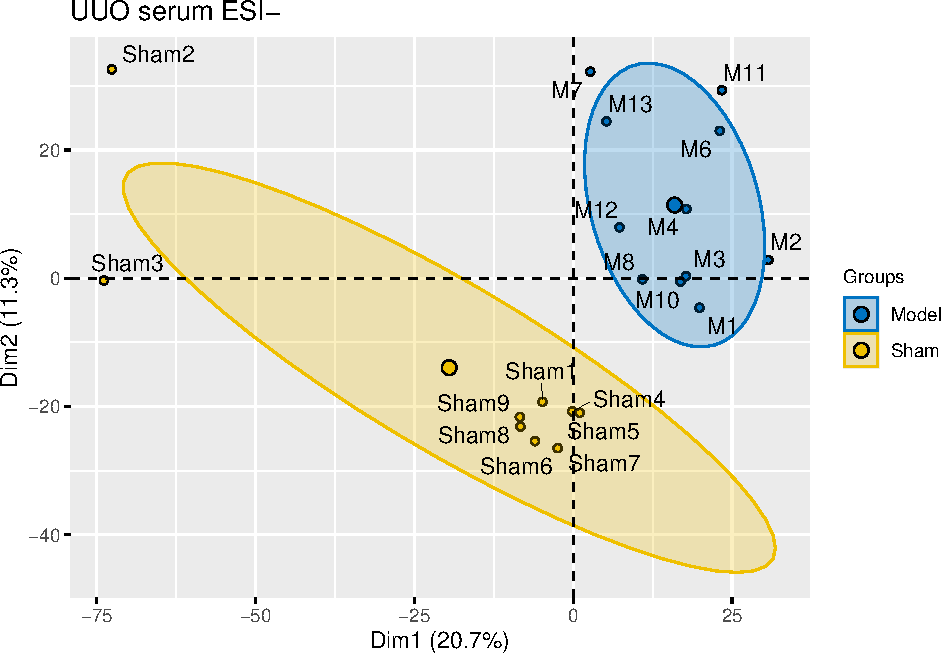
\includegraphics[keepaspectratio]{QC_report_files/figure-latex/unnamed-chunk-8-1.pdf}}

\end{document}
